\section{Кластеризация новостей}
\subsection{Векторное представление новости} \label{ssec:vectorization}
Чтобы иметь возможность группировать новости по сюжетами нам необходим метод, позволяющий сравнивать новостные документы. Сравнение двух новостей в текстовой форме невозможно, поэтому необходимо работать с их представлением в векторной форме, допускающей такие сравнения.

Наиболее популярной формой такого представления является представление <<мешком слов>>~--- то есть вектором $\vect{x}$, где каждая компонента соответствует определённому слову, входящему в данную новость $x$ \cite{frakes92}.

Однако же у такой модели есть недостаток: при представлении текста как <<мешка слов>> теряется контекст. Например, документы <<кролик быстрее, чем черепаха>> и <<черепаха быстрее, чем кролик>> имеют одинаковое векторное представление.

Простейшей характеристикой слова, которую можно использовать в данном представлении, является частота вхождения слова (от англ. TF~--- term frequency) в новость:
\begin{equation} \label{eq:tf}
    tf_{w,x}=\frac{n_{w,x}}{|x|},
\end{equation}
\begin{conditions}
    $|x|$ & длина новости $x$ (количество слов в ней); \\
    $n_{w,x}$ & количество вхождений слова $w$ в новость $x$. \\
\end{conditions}

Однако данная характеристика обладает существенным недостатком: популярные слова имеют больший вес по сравнению с менее популярными словами, что понижает качество кластеризации. Для решения этой проблемы вводят обратную частоту документа.

Обратная частота документа (от англ. IDF~--- inverse document frequency)~--- инверсия частоты, с которой слово встречается в документах. Учёт IDF уменьшает вес широкоупотребительных слов.
\begin{equation} \label{eq:idf}
    idf_w=\log\frac{N}{N_w},
\end{equation}
\begin{conditions}
    $N$ & количество новостей в коллекции;\\
    $N_w$ & количество новостей, содержащих слово $w$, $N_w=|\{x: x\ni w\}|$.
\end{conditions}

Объединяя (\ref{eq:tf}) и (\ref{eq:idf}), получаем TF-IDF характеристику:
\begin{equation} \label{eq:tf-idf}
    tf\text{-}idf_{w,x}=tf_{w,x}\cdot idf_w
\end{equation}

Векторное представление для новости $x$ в данном случае принимает вид:
\begin{equation}
    \vect{x}=(tf\text{-}idf_{w_1,x}, \quad tf\text{-}idf_{w_2,x}, \quad ...)
\end{equation}

Теперь вес некоторого слова пропорционален количеству употребления этого слова в новости, и обратно пропорционален частоте употребления слова в других новостях коллекции.

\subsection{Предобработка}
\subsubsection{Стоп-слова}
Существование заведомо высокочастотных слов (таких как <<an>>, <<and>>, <<и>>, <<как>> и др.) ведёт к раздуванию векторного представления. При этом вклад таких слов в семантику новости минимален и не влияет на кластеризацию по сюжетам. Поэтому разумно фильтровать данные слова при переводе новости в соответствующую векторную форму.

\subsubsection{Лемматизация и стемминг} \label{sssec:stemming}
При построении векторного представления в виде <<мешка слов>> нет смысла различать формы (склонения, спряжения) одного и того же слова. Это приведёт к неоправданному разрастанию словаря, дроблению статистики, увеличению ресурсоёмкости и снижению качества модели кластеризации.

\emph{Лемматизация}~--- это приведение каждого слова в документе к его нормальной форме. В русском языке нормальными формами считаются: для существительных~--- именительный падеж, единственное число; для прилагательных~--- именительный падеж, единственное число, мужской род; для глаголов, причастий, деепричастий~--- глагол в инфинитиве.

\emph{Стемминг}~--- это более простая технология, которая состоит в отбрасывании изменяемых частей слов, главным образом, окончаний. Она не требует хранения словаря всех слов и основана на правилах морфологии языка. Недостатком стемминга является большее число ошибок.

\subsection{Меры схожести новостей} \label{ssec:similarity}
\subsubsection{Эвклидова метрика}
Эвклидова метрика~--- <<классическое>> расстояние между двумя точками в пространстве \cite{huang08}:

\begin{equation}
    d(\vect{x},\vect{y})=\sqrt{\sum_{i=1}^n(x_i-y_i)^2},
\end{equation}
где $n$~--- размерность пространства.

Эвклидова метрика является наиболее просто мерой сходства между двумя векторами, однако плохо себя показывает относительно других мер при работе с текстами \cite{strehl00} и требует вычисления квадратного корня.

\subsubsection{Косинусная мера}
Косинусная мера основана предположении о том, что направление векторов имеет большее значение, чем длина каждого вектора и расстояние между ними \cite{zhong05}.

Данный метод, как следует из названия, основывается на косинусе угла между векторами:
\begin{equation}
    sim_c(\vect{x},\vect{y})=\frac{\vect{x}\cdot\vect{y}}{\lVert\vect{x}\rVert\lVert\vect{y}\rVert}
\end{equation}

\begin{figure}[h]
    \centering
    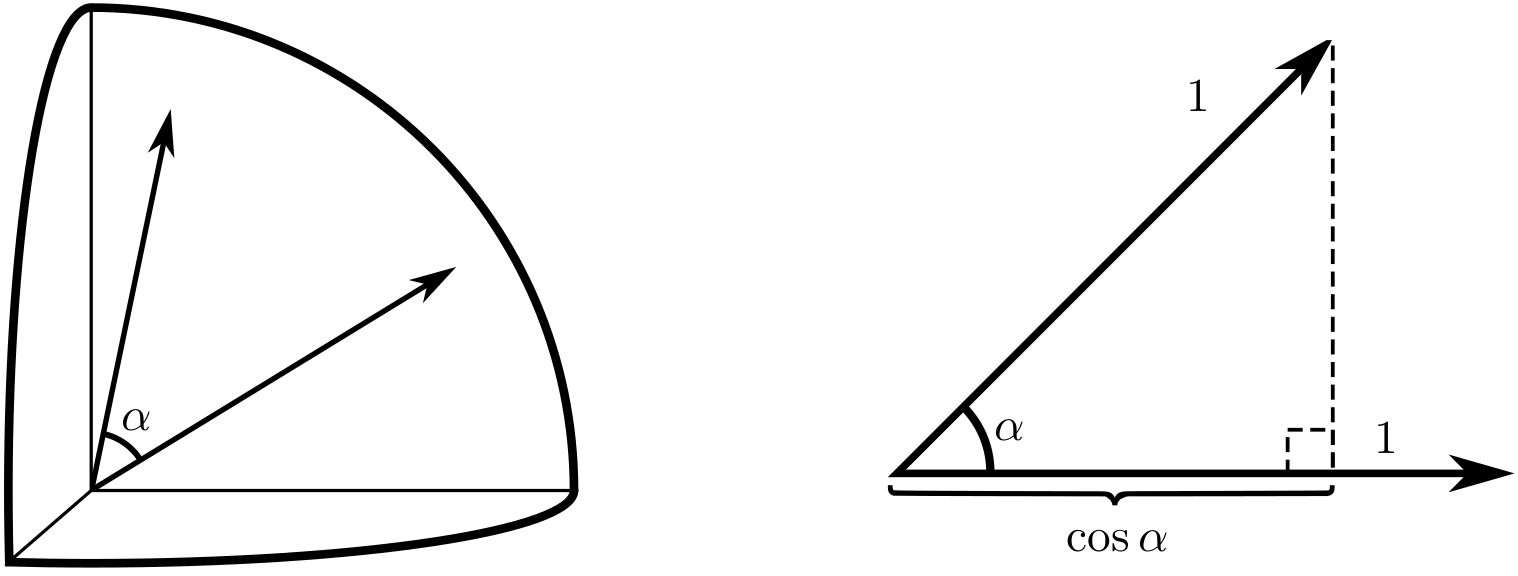
\includegraphics[width=.7\textwidth]{cosine.png}
    \caption{Косинусная мера двух единичных векторов.}
\end{figure}

В качестве длины вектора берётся эвклидова норма:
\begin{equation}
    \lVert\vect{x}\rVert=\sqrt{\vect{x}\cdot\vect{x}}
\end{equation}

Так как компоненты векторов неотрицательны исходя из выбранного представления, то значение данной меры лежит в диапазоне $[0,1]$, где значение $1$ указывает на одинаковое направление векторов, а $0$ на отсутствие общих слов.

Так как в данной мере используется только направление векторов, то достаточно работать с единичными векторами:
\begin{equation}
    \vect{\hat{x}}=\frac{\vect{x}}{\lVert\vect{x}\rVert}
\end{equation}

Таким образом, приходим к нормализованной версии косинусной меры:
\begin{equation}
    sim_c(\vect{\hat{x}},\vect{\hat{y}})=\vect{\hat{x}}\cdot\vect{\hat{y}}
\end{equation}

Что даёт возможность сильно упростить вычисления.

\subsubsection{Мера Жаккара}
Для лучшего понимания меры Жаккара сначала рассмотрим бинарный коэффициент Жаккара \cite{strehl02}:
\begin{equation}
    sim_{bj}=\frac{|S_x\cap S_y|}{|S_x\cup S_y|},
\end{equation}
где $S_x$ и $S_y$~--- множество слов в документе $x$ и $y$ соответственно.

Мера Жаккара определяется аналогично бинарному коэффициенту для случаев, когда вектора имеют не бинарные компоненты, а неотрицательные действительные значения \cite{manning09}:
\begin{equation}
    sim_j(\vect{x},\vect{y})=\frac{\vect{x}\cdot\vect{y}}{\lVert\vect{x}\rVert^2 + \lVert\vect{y}\rVert^2-\vect{x}\cdot\vect{y}}
\end{equation}

Данная мера показывает вес пересекающихся слов из обоих документов против веса слов, представленных только в одном из двух документов.

Мера Жаккара, аналогично косинусной мере, принимает значение в диапазоне $[0,1]$, где $1$ означает идентичность векторов.

\subsection{Меры схожести кластеров}
Во многих алгоритмах кластеризации предполагается объединение нескольких кластеров в один. Для этого необходимо ввести меру схожести кластеров.

\subsubsection{По ближайшему соседу}
\begin{figure}[h]
    \centering
    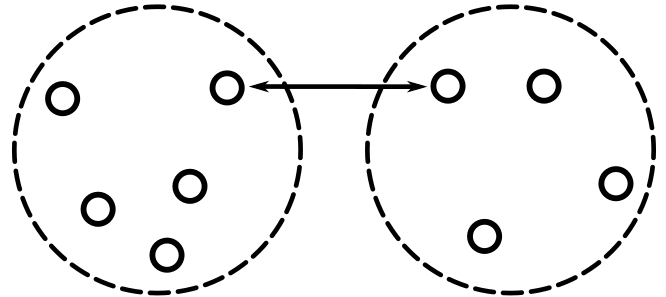
\includegraphics[width=.7\textwidth]{single-link.png}
    \caption{Мера схожести кластеров по ближайшему соседу.}
    \label{fig:single-link}
\end{figure}

Схожесть кластеров определяется как схожесть наиболее близкой пары новостей (рис.~\ref{fig:single-link}):
\begin{equation}
    sim_{near}(C_i,C_j)=\max_{x\in C_i,y\in C_j}sim(\vect{x},\vect{y}),
\end{equation}

Однако данная мера обладает существенным недостатком: создаётся цепочка связанных кластеров, каждая связанная пара который схожа по данной мере, в отличие от крайних кластеров (рис.~\ref{fig:single-link-chain}).
\begin{figure}[h]
    \centering
    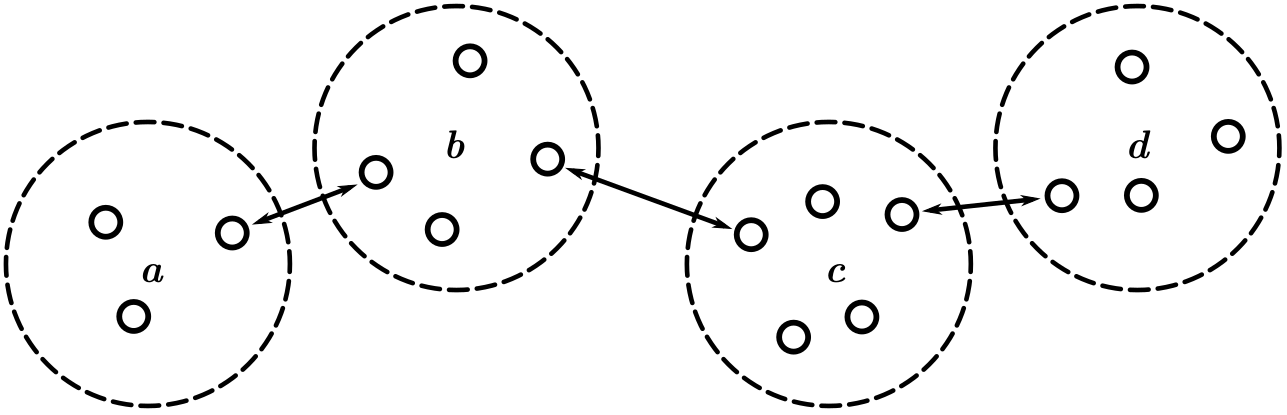
\includegraphics[width=\textwidth]{single-link-chain.png}
    \caption{Цепочка схожих кластеров.}
    \label{fig:single-link-chain}
\end{figure}

\subsubsection{По дальнему соседу}
Аналогичным образом определяется мера по самому дальнему соседу (рис.~\ref{fig:complete-link}):
\begin{equation}
    sim_{far}(C_i,C_j)=\min_{x\in C_i,y\in C_j}sim(\vect{x},\vect{y}),
\end{equation}

\begin{figure}[h]
    \centering
    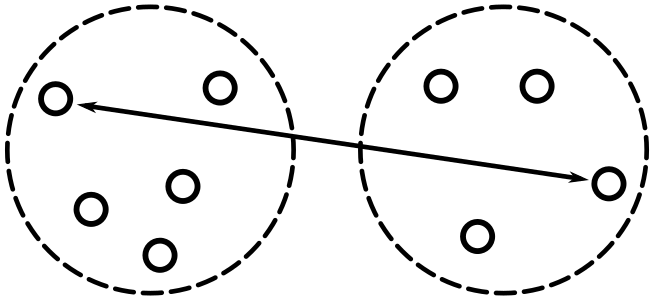
\includegraphics[width=.7\textwidth]{complete-link.png}
    \caption{Мера схожести кластеров по дальнему соседу.}
    \label{fig:complete-link}
\end{figure}

Очевидным недостатком данной меры является то, что выбросы внутри кластера сильно влияют на конечный исход кластеризации \cite{zhao05}.

\subsubsection{По средней схожести}
Мера схожести кластеров можно определять как среднюю схожесть между новостями (Unweighted Pair Group Method with Arithmetic Mean, UPGMA) \cite{lonnberg13}:
\begin{equation} \label{eq:upgma}
    sim_{upgma}(C_i,C_j)=\frac{1}{|C_i||C_j|}\sum_{\mathbf{x}\in C_i}\sum_{\mathbf{y}\in C_j}sim(\vect{x},\vect{y})
\end{equation}

\subsubsection{По среднему в группе}
Данная мера известна как Group-Average Agglomerative Clustering (GAAC) и похожа на меру по средней схожести в том смысле, что определяется среднюю схожесть между новостями. Однако здесь учитываются все пары новостей, включая входящие в один кластер \cite{zhao05}:
\begin{equation}
    sim_{gaac}(C_i,C_j)=\frac{1}{(|C_i|+|C_j|)(|C_i|+|C_j|-1)}\sum_{x\in C}\sum_{\substack{y\in C,\\x\neq y}}\vect{x}\cdot\vect{y},
\end{equation}
где $C=C_i\cup C_j$.

\subsection{Методы кластеризации}
\subsubsection{k-средних}
Метод k-средних~--- наиболее популярный метод кластеризации. Данный алгоритм требует не только новости, но ещё и количество кластеров $k$.

Основная идея заключается в том, что на каждой итерации вычисляется центр масс для каждого кластера, полученного на предыдущем шаге, затем новости разбиваются на кластеры вновь в соответствии с тем, какой из новых центров оказался ближе по выбранной метрике к векторному представлению новости:
\begin{equation}
    \vect{C}(\Omega)=\frac{1}{|\Omega|}\sum_{x\in\Omega}\vect{x},
\end{equation}
\begin{conditions}
    $\vect{C}$ & новый центр кластера; \\
    $\Omega$ & множество новостей, входящих в кластер. \\
\end{conditions}

Алгоритм завершается, когда достигается критерий останова. Обычно в качестве такого критерия берут момент, когда между итерациями состав кластеров не поменялся. При этом можно показать, что процесс завершится за конечное число итерация и зацикливание невозможно \cite{manning09}.

\subsubsection{HAC}
Hierarchical Agglomerative Clustering (HAC)~--- алгоритм иерархической кластеризации с построением иерархии снизу вверх \cite{manning09}. Первоначально создаётся по кластеру на каждую новость, после чего на каждой итерации объединяются два наиболее схожих кластеров в один. Такая процедура повторяется до тех пор, пока не останется один единственный кластер, включающий в себя все остальные. В результате получаем дерево кластеров.

\subsubsection{Разделяющий метод k-средних}
Данный метод использует два типа кластеризации: иерархическую (сверху вниз) и разделяемую \cite{steinbach00}. Алгоритм начинает работу с создания одного кластера, включающего в себя все новости. Далее каждый кластер рекурсивно делится на $k$ кластеров методом k-средних, пока не будет достигнуто заданное количество кластеров или схожесть новостей внутри кластера не достигнет заданной константы.

\subsubsection{DHCA}
Развитием алгоритма HAC является Dynamic Hierarchical Compact Algorithm (DHCA) \cite{gil05}. Данные алгоритм является онлайновым, то есть обладает способностью обрабатывать новости по мере их поступления. Стоит отметить, что результат работы алгоритма не зависит от порядка обработки новостей.

Работа алгоритма начинается с создания для каждой новости кластера, после чего строится граф $\beta$-схожести (рис.~\ref{fig:beta-similarity}), где существуют рёбра только межу кластерами схожих более, чем на $\beta$. После чего для каждой вершины оставляется только связи с максимальной схожестью. Образованные компоненты связности и будут новыми кластерами (рис.~\ref{fig:max-similarity}). После чего процесс повторяется снова, причём в качестве меры схожести между кластерами используется UPGMA (\ref{eq:upgma}).

\begin{figure}
    \centering
    \begin{subfigure}{.5\textwidth}
        \centering
        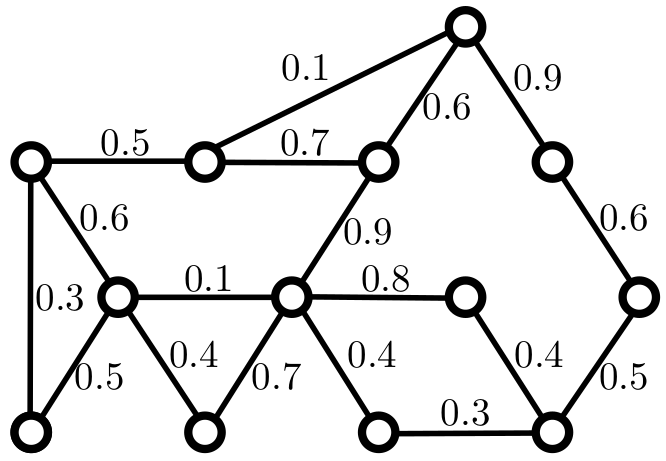
\includegraphics[width=.8\linewidth]{dhca-sim-graph.png}
        \caption{Граф $\beta$-схожести кластеров.}
        \label{fig:beta-similarity}
    \end{subfigure}%
    \begin{subfigure}{.5\textwidth}
        \centering
        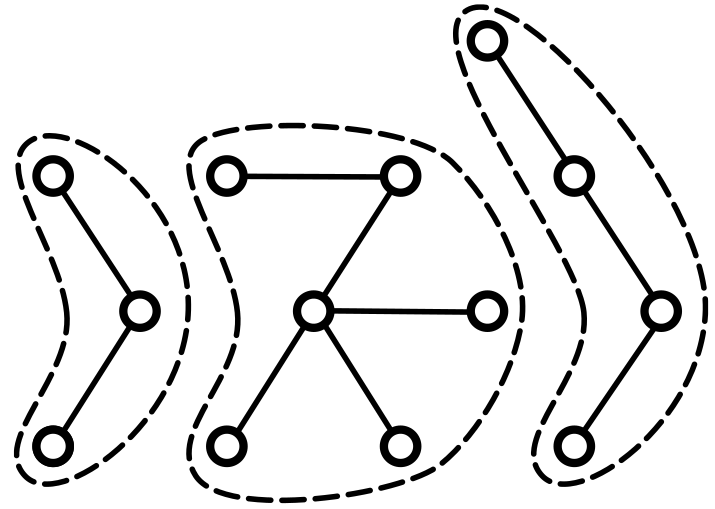
\includegraphics[width=.8\linewidth]{dhca-max-graph.png}
        \caption{Определение кластеров.}
        \label{fig:max-similarity}
    \end{subfigure}
    \caption{Пример работы DHCA.}
\end{figure}

\subsubsection{ICA}
Incremental Clustering Algorithm (ICA)~--- простой алгоритм кластеризации, позволяющий кластеризировать новости по мере их поступления \cite{lonnberg13}.

Для каждой поступающей новости находится ближайший кластер по методу UPGMA (\ref{eq:upgma}). Если схожесть с ближайшим кластером превышает заданный порог, то новость добавляется в кластер, иначе~--- создаётся новый кластер, содержащий только данную новость.

Существуют модификации данного алгоритма, позволяющие значительно сократить количество вычислений схожести кластеров \cite{lonnberg13} путём разбиения пространства кластеров.

\subsubsection{Выбор алгоритма кластеризации} \label{sssec:clustering-comparision}
Рассмотрим основные требования к алгоритму кластеризации согласно поставленной задачи:
\begin{enumerate}
    \item Алгоритм должен быть онлайновым, так как мы имеем дело с потоком новостей;
    \item В алгоритме не должно фиксироваться количество кластеров, так как каждая приходящая новость может образовывать новый сюжет, а значит и новый кластер;
    \item Должны существовать модификации алгоритма для оптимизации вычисления схожести кластеров.
\end{enumerate}

\begin{table}[ht]
    \centering
    \begin{tabular}{ l | c | c | c | c | >{\columncolor[gray]{0.8}} c }
        \hline
        & k-ср. & разд. k-ср. &  HAC & DHCA & ICA \\ \hline\hline
        Адаптивное кол-во кластеров & $-$ & $+$ & $+$ & $+$ & $+$ \\ \hline
        Иерархические кластеры      & $-$ & $+$ & $+$ & $+$ & $-$ \\ \hline
        Онлайновый алгоритм         & $-$ & $-$ & $-$ & $+$ & $+$ \\ \hline
        Возможность оптимизаций     & $+$ & $-$ & $-$ & $-$ & $+$ \\
        \hline
    \end{tabular}
    \caption{Сравнение алгоритмов кластеризации.}
    \label{tbl:clustering}
\end{table}

Исходя из требований к задаче и оценки алгоритмов (табл.~\ref{tbl:clustering}) имеет смысл выбрать ICA.
